\begin{figure}[t]
    \centering
    % \includegraphics[width=0.45\textwidth,trim={0 0 0 170mm},clip]{figures/skorch_lr_recalls_at_various_target_precisions_test.pdf}
    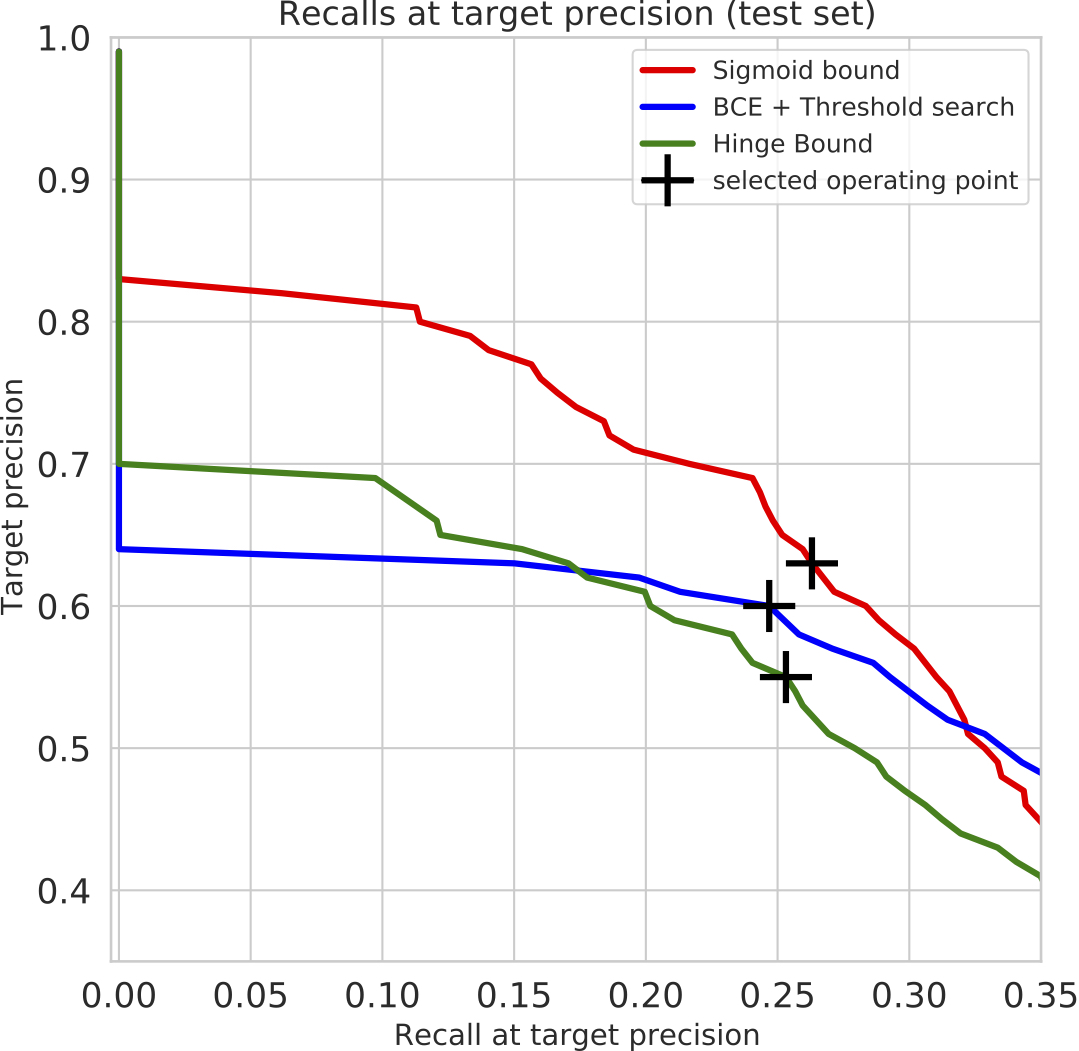
\includegraphics[width=0.9\textwidth]{content/chapters/false_alarm_control/figures/skorch_lr_recalls_at_various_target_precisions_test_mimic.jpg}
    \caption[Improvement in deployment scenario performance for predicting in-hospital mortality (in MIMIC) with our sigmoid bounds]{Predicting in-hospital mortality on MIMIC in a deployable scenario (making a prediction every 12 hours), using target precisions of $\alpha=0.7$ on train and $\alpha'=0.6$ on valid. Our proposed sigmoid bound improves precision by 0.026 (100's of fewer false alarms across the 6895 patient-stays in the test set), and improves recall by 0.01 (100's more truly at-risk patients identified).
    % Note that on lower target precisions, the sigmoid bound achieves a poorer recall, because our model is trained with the objective of maximizing recall with a minimum precision of $\alpha=0.7$.
    }%endcaption
    \label{fig:results_per_stay_slice_mimic}
    \vspace{-2.5mm}
\end{figure}
